% !Mode:: "TeX:UTF-8"	% read in as utf8 file.


\chapter{Shape Function}

\section{Introduction}
The finite element (FE) method is such an important part of most any mechanical analysis that it justifies a review of how to compute from FE results.

The usual FE notation will be used.  In particular, $ \mathbf{u} = (u,v,w) $ where $ u, v $, and $ w $ are the $ X, Y $, and $ Z $ components of the displacement of any given node.

As usual, we'll start with 2-D examples to explain the concepts before going to 3-D.

\section{Simplest 2-D Case}
The simplest case is when the element is aligned with the global coordinate system.This is in fact such a special/simple case that it is not really how FE programs are designed because they must be set-up to handle the most complex cases instead. Nevertheless, this is a good place to start for explanation purposes.

\subsection{Shape Functions}
Note that the element in this example is $ 2 \times 2 $, not $ 1 \times 1 $.  This is normal FE convention.  The displacements at any point within the element are based on the displacements of the four nodes and are arrived at by linear interpolation.

\begin{figure}[h]
\centering
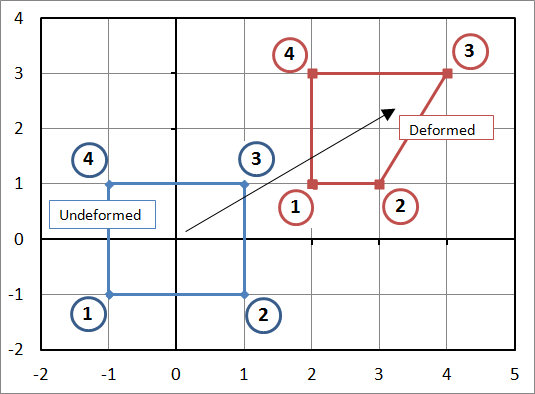
\includegraphics[width=0.7\linewidth]{figure/FE_mapping_example}
\caption{}
\label{fig:FE_mapping_example}
\end{figure}

\begin{eqnarray*}
u(X,Y) & = & {1\over 4}(1-X)(1-Y)u_1 + {1\over 4}(1+X)(1-Y)u_2 + {1\over 4}(1+X)(1+Y)u_3 + {1\over 4}(1-X)(1+Y)u_4 \\
\\
v(X,Y) & = & {1\over 4}(1-X)(1-Y)v_1 + {1\over 4}(1+X)(1-Y)v_2 + {1\over 4}(1+X)(1+Y)v_3 + {1\over 4}(1-X)(1+Y)v_4 \\
\end{eqnarray*}

where $ u(X,Y) $ is the displacement in the x-direction as a function of $ X $ and $ Y $,  $ v(X,Y) $ is the displacement in the y-direction, and $ u_1, v_1, u_2, v_2 $ etc., are the $ x $ and $ y $ displacements at nodes 1, 2, etc.

The equations are often written in shorthand as

\begin{eqnarray*}
u(X,Y) & = & \phi_1(X,Y) u_1 +  \phi_2(X,Y) u_2 +  \phi_3(X,Y) u_3 +  \phi_4(X,Y) u_4
\\
v(X,Y) & = & \phi_1(X,Y) v_1 +  \phi_2(X,Y) v_2 +  \phi_3(X,Y) v_3 +  \phi_4(X,Y) v_4
\end{eqnarray*}

where $ \phi_1(X,Y) = (1 - X)(1 - Y)/4 $ and $ \phi_2(X,Y) = (1 + X)(1 - Y)/4 $, etc. These are called <i>shape functions</i>.  Note that each shape function equals 1 at the location of its node, and zero at all other node locations.

This figure shows Shape Function \#4, for example. This shape function is $ \phi_4(X,Y) = (1 - X)(1 + Y)/4 $.  It equals 1 at (-1,1) and zero at  all other nodes.

\begin{figure}[h]
\centering
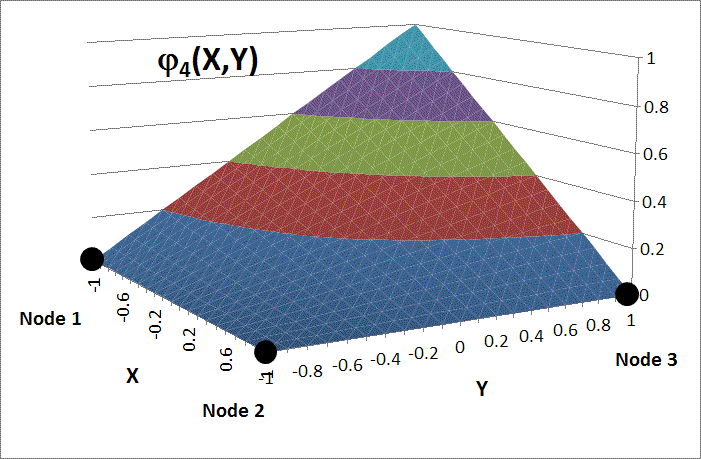
\includegraphics[width=0.7\linewidth]{figure/shape_function_4}
\caption{}
\label{fig:shape_function_4}
\end{figure}

Evaluating these equations for several special cases can help to better understand them.  For starters, evaluate them at the center of the element: $ X=0, Y=0 $.

\begin{eqnarray*}
u(0,0) & = & { u_1 + u_2 + u_3 + u_4 \over 4 }
\\
v(0,0) & = & { v_1 + v_2 + v_3 + v_4 \over 4 }
\end{eqnarray*}

Since the center is equidistant from all four nodes, each one gets equal weighting.

Also, the displacements midway between nodes 1 and 2 can be obtained
by setting $ X=0 $ and $ Y = -1 $.  This gives

\begin{eqnarray*}
u(0,-1) & = & { u_1 + u_2 \over 2 }
\\
v(0,-1) & = & { v_1 + v_2 \over 2 }
\end{eqnarray*}

And setting $ X = 0.8 $ and $ Y = 0.8 $ calculates the displacement close to node \#3.

\begin{eqnarray*}
u(0.8,0.8) & = & 0.01 u_1 + 0.09 u_2 + 0.81 u_3 + 0.09 u_4\\
v(0.8,0.8) & = & 0.01 v_1 + 0.09 v_2 + 0.81 v_3 + 0.09 v_4
\end{eqnarray*}

The closest node gets the greatest weighting and the farthest node gets the least weighting.

\subsection{Node Displacement Example}
The displacements of the nodes in the figure are

\begin{figure}[h]
\centering
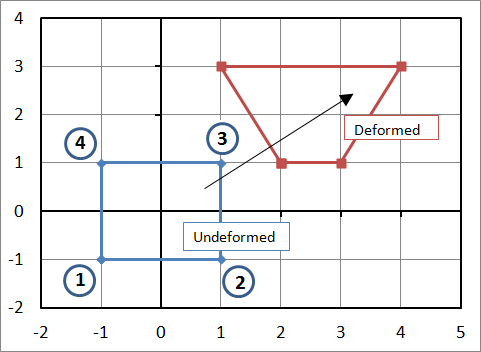
\includegraphics[width=0.7\linewidth]{figure/simple_fe_mapping_example}
\caption{}
\label{fig:simple_fe_mapping_example}
\end{figure}

\begin{eqnarray*}
u_1 = 3 \qquad u_2 = 2 \qquad u_3 = 3 \qquad u_4 = 2 \\
v_1 = 2 \qquad v_2 = 2 \qquad v_3 = 2 \qquad v_4 = 2
\end{eqnarray*}

So the displacement of a point at $ \mathbf{ X} = (0.75,0.50) $ is

\begin{eqnarray*}
u(0.75,0.50) & = & {1\over 4}[(1\text{-}0.75)(1\text{-}0.50)u_1 \text{+} (1\text{+}0.75)(1\text{-}0.50)u_2 \text{+} (1\text{+}0.75)(1\text{+}0.50)u_3 \text{+} (1\text{-}0.75)(1\text{+}0.50)u_4] \\
\\
v(0.75,0.50) & = & {1\over 4}[(1\text{-}0.75)(1\text{-}0.50)v_1 \text{+} (1\text{+}0.75)(1\text{-}0.50)v_2 \text{+} (1\text{+}0.75)(1\text{+}0.50)v_3 \text{+} (1\text{-}0.75)(1\text{+}0.50)v_4] \\
\end{eqnarray*}

which simplifies to

\begin{eqnarray*}
u(0.75,0.50) & = & 0.0313 u_1 + 0.2188 u_2 + 0.6563 u_3 + 0.0938 u_4
\\
v(0.75,0.50) & = & 0.0313 v_1 + 0.2188 v_2 + 0.6563 v_3 + 0.0938 v_4
\end{eqnarray*}

It's clear that the displacement of node \#3 gets the highest weighting because the coordinates $ (0.75, 0.50) $ are closest to it.

Substituting in the u's and v's gives

\begin{eqnarray*}
u(0.75,0.50) & = & 0.0313 * 3 + 0.2188 * 2 + 0.6563 * 3 + 0.0938 * 2 \\
	     & = & 2.688 \\
\\
v(0.75,0.50) & = & 0.0313 * 2 + 0.2188 * 2 + 0.6563 * 2 + 0.0938 * 2 \\
& = & 2
\end{eqnarray*}

So $ \mathbf{ u} = (2.688, 2) $.  The x-component is closer to 3 than 2 because the point itself is close to Node \#3, which had $ u_3 = 3 $. The y-component is 2 because all the nodes move vertically that same amount.

\subsection{FE Deformation Gradients}
Recall that the deformation gradient in terms of $ \mathbf{ u} $ is

\begin{equation*}
\mathbf{ F} = \mathbf{ I} + {\partial \mathbf{ u} \over \partial \mathbf{ X}}
\end{equation*}

The individual components of $ \mathbf{ F} $ are

\begin{eqnarray*}
F_{11} & = & {1 \over 4} [-(1-Y)u_1 + (1-Y)u_2 + (1+Y)u_3 - (1+Y)u_4] + 1 \\
\\
F_{12} & = & {1 \over 4} [-(1-X)u_1 - (1+X)u_2 + (1+X)u_3 + (1-X)u_4] \\
\\
F_{21} & = & {1 \over 4} [-(1-Y)v_1 + (1-Y)v_2 + (1+Y)v_3 - (1+Y)v_4] \\
\\
F_{22} & = & {1 \over 4} [-(1-X)v_1 - (1+X)v_2 + (1+X)v_3 + (1-X)v_4] + 1 \\
\end{eqnarray*}

Note that the deformation gradient varies throughout the element. It is not constant. This is actually a big advantage of quadrilaterals (and bricks in 3-D) over linear triangles (and tetrahedrals in 3-D). The deformation gradient in a linear triangle or tetrahedral does not vary from location to location. This tends to make them respond with artificially (and incorrectly) elevated stiffnesses.

\subsection{Simple FE Deformation Gradient}
The displacements of the nodes in the figure are

\begin{eqnarray*}
u_1 = 3 \qquad u_2 = 2 \qquad u_3 = 3 \qquad u_4 = 2 \\
v_1 = 2 \qquad v_2 = 2 \qquad v_3 = 2 \qquad v_4 = 2
\end{eqnarray*}

The deformation gradient at point $ \mathbf{ X} = (0.75,0.50) $ is

\begin{eqnarray*}
F_{11} & = & {1 \over 4} [-(1-Y)u_1 + (1-Y)u_2 + (1+Y)u_3 - (1+Y)u_4] + 1 \\
\\
       & = & 0.25 [ -(0.50)(3) + (0.50)(2) + (1.50)(3) - (1.50)(2) ] + 1\\
\\
       & = & 1.250 \\
\\
\\
F_{12} & = & {1 \over 4} [-(1-X)u_1 - (1+X)u_2 + (1+X)u_3 + (1-X)u_4] \\
\\
       & = & 0.25 [ -(0.25)(3) - (1.75)(2) + (1.75)(3) + (0.25)(2) ] \\
\\
       & = & 0.375 \\
\\
\\
F_{21} & = & {1 \over 4} [-(1-Y)v_1 + (1-Y)v_2 + (1+Y)v_3 - (1+Y)v_4] \\
\\
       & = & 0.25 [ -(0.50)(2) + (0.50)(2) + (1.50)(2) - (1.50)(2) ] \\
\\
       & = & 0.000 \\
\\
\\
F_{22} & = & {1 \over 4} [-(1-X)v_1 - (1+X)v_2 + (1+X)v_3 + (1-X)v_4] + 1 \\
\\
       & = & 0.25 [ -(0.25)(2) - (1.75)(2) + (1.75)(2) + (0.25)(2) ] + 1\\
\\
       & = & 1.000
\end{eqnarray*}

So $ \mathbf{ F} $ equals

\begin{equation*}
\mathbf{ F} = 
\begin{bmatrix}
1.250 & 0.375 \\
0.000 & 1.000
\end{bmatrix}
\end{equation*}

This makes sense because the upper right corner of the element is being stretch horizontally ($ F_{11} = 1.25 $) and is also shearing ($ F_{12} = 0.375 $).

\section{General 2-D Case}
The 'simple' section above introduces all the basic concepts of calculating displacements and deformation gradients in finite elements. But it only works for elements that are perfectly aligned with the global coordinates.  This section shows the general case that occurs when the element does not line up with the global coordinate system. For example, the element may be as shown here. The undeformedcoordinates are

\begin{align*}
X_1 = -1  & \quad & X_2 = 1 & \quad & X_3 = 0 & \quad & X_4 = -1 \\
Y_1 = -1  & \quad & Y_2 = 0 & \quad & Y_3 = 2 & \quad & Y_4 = ~1
\end{align*}

Since the element is not aligned with the global coordinate system, the simple approach from above will not work.  Instead, it is necessary to introduce two new local coordinates, $ r $ and $ s $, that span from -1 to +1.

\begin{figure}[h]
\centering
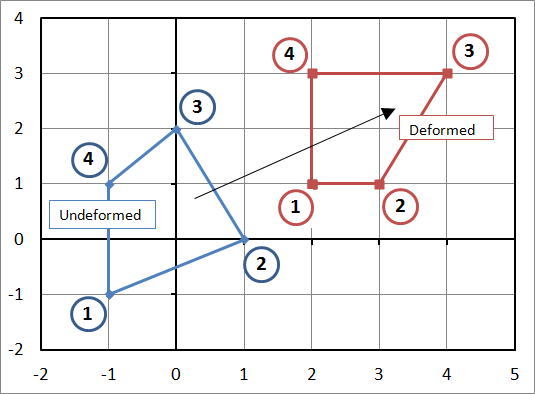
\includegraphics[width=0.7\linewidth]{figure/complex_element}
\caption{}
\label{fig:complex_element}
\end{figure}

\begin{figure}[h]
\centering
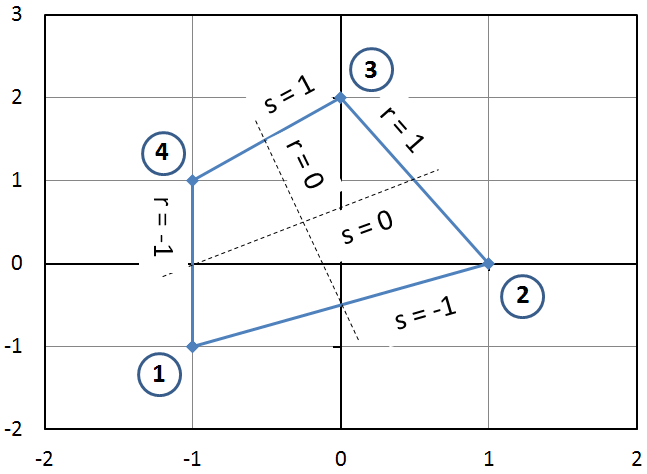
\includegraphics[width=0.7\linewidth]{figure/rs_shape_functions}
\caption{}
\label{fig:rs_shape_functions}
\end{figure}

The position within the element can be described in terms of the node coordinates and $ r $ and $ s $ as

\begin{eqnarray*}
X(r,s) & = & {1\over 4}(1-r)(1-s)X_1 + {1\over 4}(1+r)(1-s)X_2 + {1\over 4}(1+r)(1+s)X_3 + {1\over 4}(1-r)(1+s)X_4 \\
\\
\\
Y(r,s) & = & {1\over 4}(1-r)(1-s)Y_1 + {1\over 4}(1+r)(1-s)Y_2 + {1\over 4}(1+r)(1+s)Y_3 + {1\over 4}(1-r)(1+s)Y_4 \\
\end{eqnarray*}

These are the same shape functions as before, only in $ r $ and $ s $ this time. So these equations can also be written as follows

\begin{eqnarray*}
X(r,s) & = & \phi_1(r,s) X_1 +  \phi_2(r,s) X_2 +  \phi_3(r,s) X_3 +  \phi_4(r,s) X_4
\\
\\
Y(r,s) & = & \phi_1(r,s) Y_1 +  \phi_2(r,s) Y_2 +  \phi_3(r,s) Y_3 +  \phi_4(r,s) Y_4
\end{eqnarray*}

where $ \phi_1(r,s) = (1 - r)(1 - s)/4 $ and $ \phi_2(r,s) = (1 + r)(1 - s)/4 $, etc. Once again, each shape function equals 1 at the location of its node, and zero at all other node locations.

And the displacements in this example are

\begin{align*}
u_1 = 3  & \quad & u_2 = 2 & \quad & u_3 = 4 & \quad & u_4 = 3 \\
v_1 = 2  & \quad & v_2 = 1 & \quad & v_3 = 1 & \quad & v_4 = 2
\end{align*}

Just as before, the displacements within the element are interpolated using the same shape functions, but with $ r $ and $ s $.

\begin{eqnarray*}
u(r,s) & = & {1\over 4}(1-r)(1-s)u_1 + {1\over 4}(1+r)(1-s)u_2 + {1\over 4}(1+r)(1+s)u_3 + {1\over 4}(1-r)(1+s)u_4 \\
\\
v(r,s) & = & {1\over 4}(1-r)(1-s)v_1 + {1\over 4}(1+r)(1-s)v_2 + {1\over 4}(1+r)(1+s)v_3 + {1\over 4}(1-r)(1+s)v_4 \\
\end{eqnarray*}

We still need $ {\partial u \over \partial X} $ and all the other derivatives, except the challenge is that $ u $ and $ v $ are now functions of $ r $ and $ s $, not $ X $ and $ Y $.  So use the chain rule

\begin{eqnarray*}
{\partial u \over \partial X} = {\partial u \over \partial r} {\partial r \over \partial X} + {\partial u \over \partial s} {\partial s \over \partial X} \\
\\
{\partial u \over \partial Y} = {\partial u \over \partial r} {\partial r \over \partial Y} + {\partial u \over \partial s} {\partial s \over \partial Y}
\end{eqnarray*}

and similar equations exist for $ {\partial v \over \partial X} $  and  $ {\partial v \over \partial Y} $.

The complete set of equations can be written in matrix form as

\begin{align*}
\begin{bmatrix}
{\partial u \over \partial X} & {\partial u \over \partial Y} \\
\\
{\partial v \over \partial X} & {\partial v \over \partial Y} 
\end{bmatrix}
=
\begin{bmatrix}
{\partial u \over \partial r} & {\partial u \over \partial s} \\
\\
{\partial v \over \partial r} & {\partial v \over \partial s} 
\end{bmatrix}
\begin{bmatrix}
{\partial r \over \partial X} & {\partial r \over \partial Y} \\
\\
{\partial s \over \partial X} & {\partial s \over \partial Y} 
\end{bmatrix}
\end{align*}

The $ {\partial u \over \partial r} $  and  $ {\partial u \over \partial s} $ terms, and the others in the first matrix are easy. They are

\begin{eqnarray*}
{\partial u \over \partial r} & = & {1 \over 4} [-(1-s)u_1 + (1-s)u_2 + (1+s)u_3 - (1+s)u_4]  \\
\\
{\partial u \over \partial s} & = & {1 \over 4} [-(1-r)u_1 - (1+r)u_2 + (1+r)u_3 + (1-r)u_4]
\end{eqnarray*}

However, the $ {\partial r \over \partial X} $  and  $ {\partial s \over \partial X} $ terms in the second matrix are trickier because $ r $ and $ s $ are not explicitly functions of $ X $ and $ Y $.  It's the other way around. Fortunately, the needed terms are just the inverse of a certain matrix. It is

\begin{eqnarray*}
\begin{bmatrix}
{\partial r \over \partial X} & {\partial r \over \partial Y} \\
\\
{\partial s \over \partial X} & {\partial s \over \partial Y} 
\end{bmatrix}
=
\begin{bmatrix}
{\partial X \over \partial r} & {\partial X \over \partial s} \\
\\
{\partial Y \over \partial r} & {\partial Y \over \partial s} 
\end{bmatrix}^{-1}
\end{eqnarray*}

And this matrix is easy to compute and then take the numerical inverse of.
So the entire process can be written as

\begin{eqnarray*}
\begin{bmatrix}
{\partial u \over \partial X} & {\partial u \over \partial Y} \\
\\
{\partial v \over \partial X} & {\partial v \over \partial Y} 
\end{bmatrix}
=
\begin{bmatrix}
{\partial u \over \partial r} & {\partial u \over \partial s} \\
\\
{\partial v \over \partial r} & {\partial v \over \partial s} 
\end{bmatrix}
\begin{bmatrix}
{\partial X \over \partial r} & {\partial X \over \partial s} \\
\\
{\partial Y \over \partial r} & {\partial Y \over \partial s} 
\end{bmatrix}^{-1}
\end{eqnarray*}

\subsection{Complex Example}
So now we can complete the example of the arbitrarily shaped element being deformed. Recall that the coordinates are

\begin{align*}
X_1 = -1  & \quad & X_2 = 1 & \quad & X_3 = 0 & \quad & X_4 = -1 \\
Y_1 = -1  & \quad & Y_2 = 0 & \quad & Y_3 = 2 & \quad & Y_4 = ~1
\end{align*}

and the displacements are

\begin{align*}
u_1 = 3  & \quad & u_2 = 2 & \quad & u_3 = 4 & \quad & u_4 = 3 \\
v_1 = 2  & \quad & v_2 = 1 & \quad & v_3 = 1 & \quad & v_4 = 2
\end{align*}

Let's compute the deformation gradient at the centroid of the element, where $ r = s = 0 $. First, the centroid itself is at

\begin{align*}
X_{cg} \; & = & \; {1 \over 4} (X_1 + X_2 + X_3 + X_4) \; & = & \; {1 \over 4} (-1 + 1 + 0 - 1) \; & = & \; -0.25
\\
\\
Y_{cg} \; & = & \; {1 \over 4} (Y_1 \, + Y_2 \, + Y_3 \, + Y_4) \; & = & \; {1 \over 4} (-1 + 0 + 2 + 1) \; & = & \; \;\; 0.50
\end{align*}

And we can calculate $ u $ and $ v $ in order to determine where the centroid ends up. This step is not really necessary, but we'll do it anyway.

\begin{align*}
u_{cg} \; & = & \; {1 \over 4} (u_1 + u_2 + u_3 + u_4) \; & = & \; {1 \over 4} (3 + 2 + 4 + 3) \; & = & \; 3.0
\\
\\
v_{cg} \; & = & \; {1 \over 4} (v_1 + v_2 + v_3 + v_4) \; & = & \; {1 \over 4} (2 + 1 + 1 + 2) \; & = & \; 1.5
\end{align*}

So $ x_{cg} = -0.25 + 3 = 2.75 $ and $ y_{cg} = 0.5 + 1.5 = 2.0 $.

The next step in calculating $ \mathbf{ F} $ is to compute $ {\partial u \over \partial r} $, $ {\partial u \over \partial s} $, and all the other terms at the centroid.

\begin{align*}
\left. {\partial u \over \partial r}\right|_{0,0} \; & = & \; {1 \over 4} (-u_1 + u_2 + u_3 - u_4) \; & = & \; {1 \over 4} (-3 + 2 + 4 - 3) \; & = \;\; 0.0 \\
\\
\\
\left. {\partial u \over \partial s}\right|_{0,0} \; & = & \; {1 \over 4} (-u_1 - u_2 + u_3 + u_4) \; & = & \; {1 \over 4} (-3 - 2 + 4 + 3) \; & = \;\; 0.5 \\
\\
\\
\left. {\partial v \over \partial r}\right|_{0,0} \; & = & \; {1 \over 4} (-v_1 + v_2 + v_3 - v_4) \; & = & \; {1 \over 4} (-2 + 1 + 1 - 2) \; & = -0.5 \\
\\
\\
\left. {\partial v \over \partial s}\right|_{0,0} \; & = & \; {1 \over 4} (-v_1 - v_2 + v_3 + v_4) \; & = & \; {1 \over 4} (-2 - 1 + 1 + 2) \; & = \;\; 0.0
\end{align*}

So the matrix of partial derivatives of the displacement field is

\begin{eqnarray*}
\begin{bmatrix}
{\partial u \over \partial r} & {\partial u \over \partial s} \\
\\
{\partial v \over \partial r} & {\partial v \over \partial s} 
\end{bmatrix}
=
\begin{bmatrix}
0 & 0.5 \\
\\
-0.5 & 0 
\end{bmatrix}
\end{eqnarray*}

The partial derivatives of the node coordinates are

\begin{align*}
\left. {\partial X \over \partial r}\right|_{0,0} \; & = & \; {1 \over 4} (-X_1 + X_2 + X_3 - X_4) \; & = & \; {1 \over 4} ( 1 + 1 + 0 + 1) \; & = \;\; 0.75 \\
\\
\\
\left. {\partial X \over \partial s}\right|_{0,0} \; & = & \; {1 \over 4} (-X_1 - X_2 + X_3 + X_4) \; & = & \; {1 \over 4} ( 1 - 1 + 0 - 1) \; & =  -0.25 \\
\\
\\
\left. {\partial Y \over \partial r}\right|_{0,0} \; & = & \; {1 \over 4} (-Y_1 + Y_2 + Y_3 - Y_4) \; & = & \; {1 \over 4} ( 1 + 0 + 2 - 1) \; & = \;\; 0.50 \\
\\
\\
\left. {\partial Y \over \partial s}\right|_{0,0} \; & = & \; {1 \over 4} (-Y_1 - Y_2 + Y_3 + Y_4) \; & = & \; {1 \over 4} ( 1 - 0 + 2 + 1) \; & = \;\; 1.0
\end{align*}

The matrix of partial derivatives of the coordinates is

\begin{eqnarray*}
\begin{bmatrix}
{\partial X \over \partial r} & {\partial X \over \partial s} \\
\\
{\partial Y \over \partial r} & {\partial Y \over \partial s} 
\end{bmatrix}
=
\begin{bmatrix}
0.75 & -0.25 \\
\\
0.50 & \;\; 1.00
\end{bmatrix}
\end{eqnarray*}

And the inverse is

\begin{eqnarray*}
\begin{bmatrix}
{\partial X \over \partial r} & {\partial X \over \partial s} \\
\\
{\partial Y \over \partial r} & {\partial Y \over \partial s} 
\end{bmatrix}^{-1}
=
\begin{bmatrix}
\;\;\; 1.1429 & 0.2857 \\
\\
-0.5714 & 0.8571
\end{bmatrix}
\end{eqnarray*}

So

\begin{align*}
\begin{bmatrix}
{\partial u \over \partial X} & {\partial u \over \partial Y} \\
\\
{\partial v \over \partial X} & {\partial v \over \partial Y} 
\end{bmatrix}
=
\begin{bmatrix}
\;\;\;0 & 0.5 \\
\\
-0.5 & 0.0
\end{bmatrix}
\begin{bmatrix}
\;\;\; 1.1429 & 0.2857 \\
\\
-0.5714 & 0.8571
\end{bmatrix}
=
\begin{bmatrix}
-0.2857 & 0.4286 \\
-0.5715 & -0.1429
\end{bmatrix}
\end{align*}

And adding $ \mathbf{ I} $ to get $ \mathbf{ F} $ finally gives

\begin{equation*}
\mathbf{ F} = 
\begin{bmatrix}
 0.7143 & 0.4286 \\
\\
-0.5715 & 0.8572
\end{bmatrix}
\end{equation*}

And a polar decomposition can be applied to find

\begin{equation*}
\mathbf{ R} = 
\begin{bmatrix}
 \;\;\; 0.844 & 0.537 \\
\\
-0.537 & 0.844
\end{bmatrix}
\qquad \qquad
\mathbf{ U} = 
\begin{bmatrix}
 \;\;\; 0.909 & -0.099 \\
\\
-0.099 & \;\;\; 0.953
\end{bmatrix}
\end{equation*}

So this central portion of the element rotates

\begin{equation*}
\theta \quad = \quad \text{Sin}^{-1}(-0.537) \quad = \quad -32.5^\circ
\end{equation*}

And the horizontal part of the element is compressed ~9\%, the vertical part is compressed ~5\%, and it is sheared -20\%.  These results may be intuitive whenever the element is originally aligned with the global coordinate system, however that does not seem to be the case when the element is randomly oriented.

\subsection{Isoparametric Elements}
So, given $ r $ and $ s $, the $ (X,Y) $ coordinates in the element can be calculated using

\begin{eqnarray*}
X(r,s) & = & \phi_1(r,s) X_1 +  \phi_2(r,s) X_2 +  \phi_3(r,s) X_3 +  \phi_4(r,s) X_4
\\
Y(r,s) & = & \phi_1(r,s) Y_1 +  \phi_2(r,s) Y_2 +  \phi_3(r,s) Y_3 +  \phi_4(r,s) Y_4
\end{eqnarray*}

and the displacements $ (u,v) $ can be calculated using the exact same shape functions

\begin{eqnarray*}
u(r,s) & = & \phi_1(r,s) u_1 +  \phi_2(r,s) u_2 +  \phi_3(r,s) u_3 +  \phi_4(r,s) u_4
\\
v(r,s) & = & \phi_1(r,s) v_1 +  \phi_2(r,s) v_2 +  \phi_3(r,s) v_3 +  \phi_4(r,s) v_4
\end{eqnarray*}

The fact that the same shape functions are used for both coordinates and displacements is what makes this an \textit{isoparametric element}. This makes life much easier than if they are different.

\section{3-D Case}
The 3-D case follows all the same principles of the 2-D examples above, except the shape functions change as follows.

\begin{eqnarray*}
u(r,s,t) & \; = \; & {1\over 8}(1-r)(1-s)(1-t)u_1 \; + \; {1\over 8}(1+r)(1-s)(1-t)u_2 \; + \\
\\
         &   & {1\over 8}(1+r)(1+s)(1-t)u_3 \; + \; {1\over 8}(1-r)(1+s)(1-t)u_8 \; + \\
\\
	 &   & {1\over 8}(1-r)(1-s)(1+t)u_5 \; + \; {1\over 8}(1+r)(1-s)(1+t)u_6 \; + \\
\\
	 &   & {1\over 8}(1+r)(1+s)(1+t)u_7 \; + \; {1\over 8}(1-r)(1+s)(1+t)u_8
\end{eqnarray*}

The equations for the $ v $ and $ w $ displacements are the same, as well as the coordinate interpolation equations for $ X $, $ Y $, and $ Z $.

\subsection{Triangles}
Linear Triangles and tetrahedrons deserve special attention, not because of any good qualities, but because of their significantly bad qualities that make them a very poor choice for use.  But it should be stressed that these limitations only apply to linear elements. Quadratic triangles and tetrahedrons are excellent elements.

\begin{figure}[h]
\centering
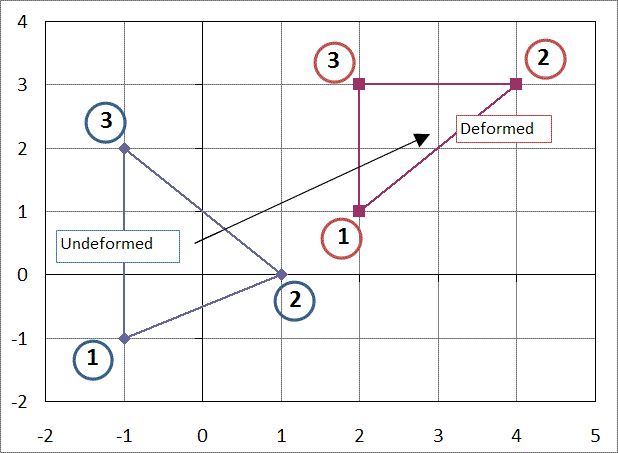
\includegraphics[width=0.7\linewidth]{figure/triangle_element}
\caption{}
\label{fig:triangle_element}
\end{figure}

The shape functions for triangles are

\begin{eqnarray*}
X(r,s) & \; = \; & r X_1 \; + \; s X_2 \; + \; (1 - r - s) X_3 \\
\\
Y(r,s) & \; = \; & r Y_1 \; + \; s Y_2 \; + \; (1 - r - s) Y_3 \\
\end{eqnarray*}

for the coordinates and 

\begin{eqnarray*}
u(r,s) & \; = \; & r u_1 \; + \; s u_2 \; + \; (1 - r - s) u_3 \\
\\
v(r,s) & \; = \; & r v_1 \; + \; s v_2 \; + \; (1 - r - s) v_3 \\
\end{eqnarray*}

for the displacements.

The derivatives are easy in this case.  Recall that

\begin{eqnarray*}
\begin{bmatrix}
{\partial u \over \partial X} & {\partial u \over \partial Y} \\
\\
{\partial v \over \partial X} & {\partial v \over \partial Y} 
\end{bmatrix}
=
\begin{bmatrix}
{\partial u \over \partial r} & {\partial u \over \partial s} \\
\\
{\partial v \over \partial r} & {\partial v \over \partial s} 
\end{bmatrix}
\begin{bmatrix}
{\partial X \over \partial r} & {\partial X \over \partial s} \\
\\
{\partial Y \over \partial r} & {\partial Y \over \partial s} 
\end{bmatrix}^{-1}
\end{eqnarray*}

Applying the derivatives to the triangle shape functions results in

\begin{eqnarray*}
\begin{bmatrix}
{\partial u \over \partial X} & {\partial u \over \partial Y} \\
\\
{\partial v \over \partial X} & {\partial v \over \partial Y} 
\end{bmatrix}
=
\begin{bmatrix}
u_1 - u_3 & u_2 - u_3 \\
\\
v_1 - v_3 & v_2 - v_3 \\
\end{bmatrix}
\begin{bmatrix}
X_1 - X_3 & X_2 - X_3 \\
\\
Y_1 - Y_3 & Y_2 - Y_3 \\
\end{bmatrix}^{-1}
\end{eqnarray*}

The key revelation here is that the result is independent of $ r $ and $ s $, which means that it is constant throughout the element. This constancy is the problem, for it tends to make triangles react much too stiff in FE analyses.  Because of this, they should be avoided (just the linear ones, not the quadratics, which are fine) whenever possible. Although it is recognized that a few are almost always necessary anyway.

\subsection{Tetrahedrals}
3-D linear tetrahedrons have the exact same problem as 2-D linear triangles.

The shape functions for linear tetrahedrons are

\begin{eqnarray*}
X(r,s,t) & \; = \; & r X_1 \; + \; s X_2 \; + \; t X_3 \; + \; (1 - r - s - t) X_4 \\
\\
Y(r,s,t) & \; = \; & r Y_1 \; + \; s Y_2 \; + \; t Y_3 \; + \; (1 - r - s - t) Y_4 \\
\\
Z(r,s,t) & \; = \; & r Z_1 \; + \; s Z_2 \; + \; t Z_3 \; + \; (1 - r - s - t) Z_4 \\
\end{eqnarray*}

for the coordinates and 

\begin{eqnarray*}
u(r,s,t) & \; = \; & r u_1 \; + \; s u_2 \; + \; t u_3 \; + \; (1 - r - s - t) u_4 \\
\\
v(r,s,t) & \; = \; & r v_1 \; + \; s v_2 \; + \; t v_3 \; + \; (1 - r - s - t) v_4 \\
\\
w(r,s,t) & \; = \; & r w_1 \; + \; s w_2 \; + \; t w_3 \; + \; (1 - r - s - t) w_4 \\
\end{eqnarray*}

for the displacements.

The derivatives are also easy in this case.  The result is

\begin{eqnarray*}
\begin{bmatrix}
{\partial u \over \partial X} & {\partial u \over \partial Y}  & {\partial u \over \partial Z} \\
\\
{\partial v \over \partial X} & {\partial v \over \partial Y}  & {\partial v \over \partial Z} \\
\\
{\partial w \over \partial X} & {\partial w \over \partial Y}  & {\partial w \over \partial Z} \\
\end{bmatrix}
=
\begin{bmatrix}
u_1 - u_4 & u_2 - u_4 & u_3 - u_4 \\
\\
v_1 - v_4 & v_2 - v_4 & u_3 - u_4 \\
\\
w_1 - w_4 & w_2 - w_4 & u_3 - u_4 \\
\end{bmatrix}
\begin{bmatrix}
X_1 - X_4 & X_2 - X_4 & X_3 - X_4 \\
\\
Y_1 - Y_4 & Y_2 - Y_4 & Y_3 - Y_4 \\
\\
Z_1 - Z_4 & Z_2 - Z_4 & Z_3 - Z_4 \\
\end{bmatrix}^{-1}
\end{eqnarray*}

Once again, the result is independent of $ r $ and $ s $, and now $ t $, which means that it is constant throughout the element. Not good!